% ===================================================================
% FIGURE: Progressive De-identification Recovery (from E2 results)
% Shows l_PHI recovery as identifiers are removed one by one
% Requires: \usepackage{pgfplots} in preamble
% ===================================================================

\begin{figure}[t]
\centering
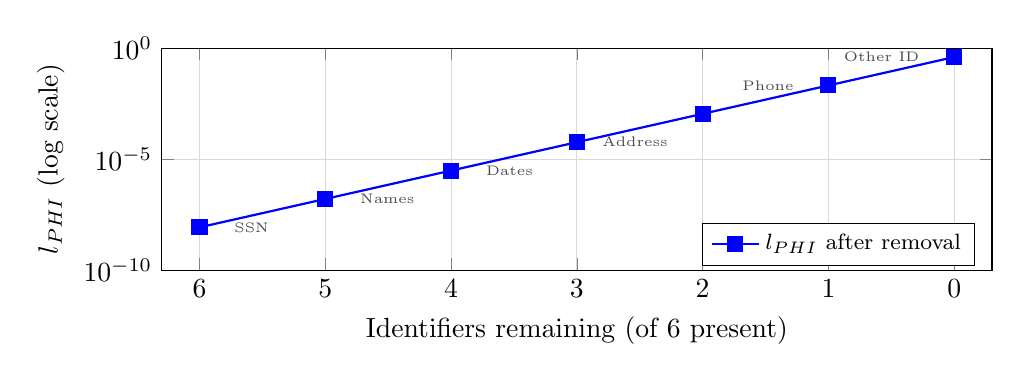
\begin{tikzpicture}
\begin{axis}[
    width=\columnwidth,
    height=4.4cm,
    xlabel={Identifiers remaining (of 6 present)},
    ylabel={$l_{\text{PHI}}$ (log scale)},
    ymode=log,
    xmin=-0.3, xmax=6.3,
    ymin=1e-10, ymax=1,
    xtick={0,1,2,3,4,5,6},
    xticklabels={0,1,2,3,4,5,6},
    x dir=reverse,
    legend style={at={(0.98,0.02)}, anchor=south east, font=\footnotesize},
    grid=major,
    grid style={gray!30},
    every axis plot/.append style={thick},
    nodes near coords style={font=\tiny, anchor=south west},
]

% Progressive de-identification data points
\addplot[blue, mark=square*, mark size=2.5pt]
    coordinates {
        (6, 8.443126e-09)
        (5, 1.604194e-07)
        (4, 3.047969e-06)
        (3, 5.791140e-05)
        (2, 1.100317e-03)
        (1, 2.090602e-02)
        (0, 3.972143e-01)
    };
\addlegendentry{$l_{\text{PHI}}$ after removal}

% Annotations for key steps
\node[font=\tiny, anchor=west, text=black!70] at (axis cs:5.8, 8.4e-09) {SSN};
\node[font=\tiny, anchor=west, text=black!70] at (axis cs:4.8, 1.6e-07) {Names};
\node[font=\tiny, anchor=west, text=black!70] at (axis cs:3.8, 3.0e-06) {Dates};
\node[font=\tiny, anchor=east, text=black!70] at (axis cs:2.2, 5.8e-05) {Address};
\node[font=\tiny, anchor=east, text=black!70] at (axis cs:1.2, 2.1e-02) {Phone};
\node[font=\tiny, anchor=east, text=black!70] at (axis cs:0.2, 3.97e-01) {Other ID};

\end{axis}
\end{tikzpicture}
\caption{Progressive de-identification of a Synthea patient record: each removal raises $l_{\text{PHI}}$ by about $19\times$ (the ratio $0.95/0.05$), from $8.44 \times 10^{-9}$ with 6 identifiers to $0.397 = 0.95^{18}$ after full removal; theory-validated at every step.}
\label{fig:progressive_deident}
\end{figure}
